\documentclass[../specifications.tex]{subfiles}

\begin{document}

  図 \ref{fig:external-interface} にプロセッサの外部インタフェースを示す.
  信号線名の後ろに \# が記述されている信号線は負論理であり, 
  \# が記述されていない信号線は正論理であることを示している.

  \begin{figure}
    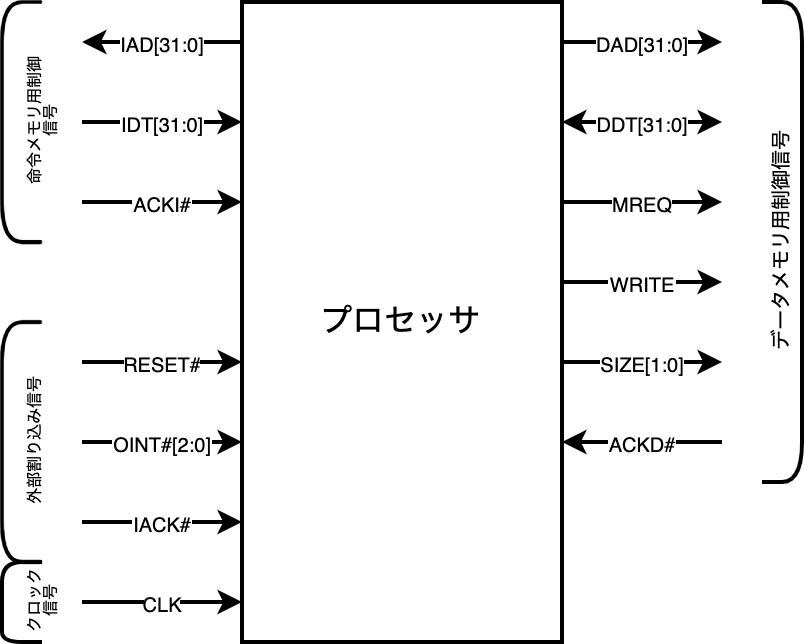
\includegraphics[scale=1.5, bb=-55 0 50 100]{../../images/external_interface.png}
    \caption{プロセッサの外部インタフェース}
    \label{fig:external-interface}
  \end{figure}

  図 \ref{fig:external-interface} にあるそれぞれの信号線の説明は以下の通りである.
  \begin{itemize}
    \item IAD (Instruction ADdress Bus)
    \newline 命令メモリへの 32 [bit] のアクセスアドレスパス.

    \item IDT (Instruction DaTa Bus)
    \newline 命令メモリからの 32 [bit] のデータパス.

    \item ACKI\# (ACKnowledge from Instruction memory)
    \newline 命令メモリへのアクセスに対するアクノリッジ信号.
    命令メモリにアクセスして, この信号がインアクティブであれば, 
    読み出し・書き込みが完了していないことを意味する.
    
    \item RESET\#
    \newline リセット信号.

    \item OINT\#
    \newline 外部からの割り込みを示す信号.
    外部からの割り込みがあった時に, 対応するビットがアクティブになる.

    \item IACK\# (Interruption ACKnowledge)
    \newline 外部の割り込みを処理している時にアクティブになる信号.

    \item CLK (CLocK)
    \newline クロック信号

    \item DAD (Data ADdress bus)
    \newline データメモリへの 32 [bit] のアクセスアドレスパス.

    \item DDT (Data DaTa bu)
    \newline データメモリからの 32 [bit] のデータパス.

    \item MREQ
    \newline データメモリに対するアクセス (読み出し・書き込み) をリクエストするための信号.
    データメモリへアクセスする前にリクエスト信号をアクティブにする必要がある.

    \item WRITE
    \newline データメモリへの書き込みをリクエストする信号.
    データメモリにデータを書き込む時にこの信号をアクティブにする必要がある.

    \item SIZE
    \newline データメモリへのアクセスサイズを示す.
    \begin{itemize}
      \item word アクセス: SIZE = 00
      \item halfword アクセス: SIZE = 01
      \item byte アクセス: SIZE = 10
    \end{itemize}

    \item ACKD\# (ACKnowledge from Data memory)
    \newline データメモリへのアクセスに対するアクノリッジ信号.
    データメモリにアクセスして, この信号がインアクティブであれば, 
    読み出し・書き込みが完了していないことを意味する.

  \end{itemize}

  命令メモリとデータメモリはシミュレーション環境で用意されているため, 
  プロセッサの中に実装しない.
  ただし, メモリはリトルエンディアン方式を採用する.
  メモリのアドレスは 1 [byte] ごとに振り分けられ, 
  1つのアドレスに 32 [bit] のデータを保持することができる.

  また, シミュレーション環境において, 外部からの割り込みが発生しないため, 
  OINT 入力信号の処理と, IACK 出力信号への出力を行わない.

\end{document}
